\documentclass[12pt,a4paper,utf8x]{report}
\usepackage [frenchb]{babel}

%\usepackage{ucs}
\usepackage{pgfgantt}
\usepackage{graphicx}
\usepackage{caption}
\usepackage[utf8x]{inputenc}
\usepackage{multicol}
\usepackage{url} % Pour avoir de belles url
\usepackage {geometry}
%\usepackage {listings} %Pour mettre du code source 
\usepackage{verbatim}
\usepackage{lscape} % Pour pouvoir passer en paysage
\usepackage{geometry}
\usepackage{pdflscape}
\usepackage{colortbl}
\usepackage[strings]{underscore}
\geometry{left=2.5cm,right=2.5cm,vmargin=2cm}
\usepackage[pdftex,bookmarks = true,bookmarksnumbered = true,pdfpagemode = None,pdfstartview = FitH,pdfpagelayout = OneColumn,colorlinks=true,linkcolor=black,urlcolor=blue,citecolor=blue,pdfborder = {0 0 0}]{hyperref}


%chapitre---------------------------------------------------------------------
 
%%%% debut macro pour enlever le nom chapitre %%%%
\makeatletter
\def\@makechapterhead#1{%
  \vspace*{50\p@}%
  {\parindent \z@ \raggedright \normalfont
    \interlinepenalty\@M
    \ifnum \c@secnumdepth >\m@ne
        \Huge\bfseries \thechapter\quad
    \fi
    \Huge \bfseries #1\par\nobreak
    \vskip 40\p@
  }}

\def\@makeschapterhead#1{%
  \vspace*{50\p@}%
  {\parindent \z@ \raggedright
    \normalfont
    \interlinepenalty\@M
    \Huge \bfseries  #1\par\nobreak
    \vskip 40\p@
  }}
\makeatother
%%%% fin macro %%%% 

\begin{document}

\begin{titlepage}
\begin{flushright}
   	
\includegraphics[scale=0.30]{univorleans.png}\\ 
   	   	Département Informatique
\end{flushright}
\vspace{30mm}
\begin{center}
\huge{Mémoire intermédiaire \\Travaux d'étude et de recherche }\\
\vspace{7mm}
\large{Sujet : \\Impact de la parallélisation d'algorithmes sur la consommation
énergétique des architectures parallèles}\\
\vspace{4mm}
\large{Proposé et encadré par : Sylvain JUBERTIE}
\vspace{4mm}
\large{\\Réalisé par :}\\
\large{Youenn LEBRAS, Romain PROU, Issam RAIS \\ et Joris RUBAGOTTI }\\
\end{center}
\begin{figure}[b!]
\begin{flushright}
~~\\ ~~\\ ~~\\ ~~\\ ~~\\ ~~\\ ~~\\
\large{Année : 2013-2014}
\end{flushright}
\end{figure}
\end{titlepage}

\tableofcontents
\clearpage

\chapter{Résumé du projet}

Notre projet, proposé par M. JUBERTIE, nous entraîne dans l'étude de l'impact de la parallélisation d'algorithmes sur la consommation énergétique des architectures parallèles.\\ 

Les machines actuelles, du smartphone aux supercalculateurs, possèdent des 
processeurs multi-c\oe{}urs. Afin d'augmenter les performances le développeur doit s'appliquer à développer des codes s'exécutant en parallèle. Cependant, la parallélisation n'est pas très répandue dans les périphériques nomades. Les nombreux c\oe{}urs servent généralement à exécuter plusieurs tâches distinctes et à diminuer la consommation 
énergétique. \\

Pour juger de l'impact du parallélisme sur consommation énergétique, certains choix s'offrent à nous  : soit faire fonctionner un seul processeur à sa fréquence 
maximale, soit les paralléliser et utiliser plusieurs c\oe{}urs à fréquence réduite. \\

Pour cela de nombreux algorithmes parallèles seront implémentés et exécutés sur différentes architectures.
Une comparaison entre des codes écrits en Java et C/C++ pour Android pourra 
également être envisagée afin d'étudier l'impact du langage sur les 
performances et la consommation. \\ 

\chapter{Introduction au domaine}

Dans un premier temps, il est important d'évoquer ce qui caractérise les architectures que nous emploierions lors de nos tests ainsi que les méthodes de parallélisation et leurs différences de fonctionnement.

\section{ Les différentes architectures }

Aujourd'hui il existe de nombreuses architectures de processeurs différentes au sein de nos machines aussi bien dans les ordinateurs que dans les appareils nomades. Nous allons explorer deux grandes familles :
les architectures ARM (Advanced RISC Machines) utilisées dans les appareils nomades et les architectures x86 (et x86-64) utilisées dans la plupart des ordinateurs.

\subsection{ Les architectures Advanced RISC Machines (ARM)}

Les architectures ARM sont introduites en 1983 mais elle ne s'insère que depuis quelques années sur le marché des appareils nomades. elles sont basés sur des architectures RISC (Reduced Instruction Set Computer) 32 bits (ARMv3 à ARMv7) et récemment 64 bits avec l'ARMv8. Aujourd'hui, le développement autour de cette architecture a atteint son apogée. On assiste à une augmentation des fréquences constante ainsi qu'au nombre de cœurs qu'un processeur possède.

\subsubsection{ Reduced Instruction Set Computer }

Comme introduit précédemment, l'architecture employée pour l'ARM est RISC. il s'agit d'un type d'architecture matérielle de microprocesseur. Elle est caractérisée par un jeu d'instructions réduit, facile à décoder et comportant uniquement des instructions simples. Elle s'oppose à l'architecture CISC (Complex Instruction Set Computer) employé sur les architectures x86 et x86-64 que nous décrirons plus tard.
\\
Ce type d'architecture est caractérisée par le fait de reposer l'optimisation du code sur le compilateur tandis que les instructions sont faciles à décoder pour le processeur. Pour cela :
\begin{itemize}
\item Ces processeurs possèdent un nombre important de registres "généraux" (un minimum de 16 et généralement de 32). Ils sont tous équivalents afin de faciliter leur allocation par le compilateur
\item Les instructions possèdent une taille fixe, souvent de 32 bits
\item Les instructions utilisées pour des calculs arithmétiques possèdent généralement 3 adresses avec 2 registres comme opérandes et un registre de sortie
\item Pour les accès à la mémoire, des instructions spécifiques sont employées et une valeur doit, au préalable, être chargée dans un registre pour être utilisée. Ce genre d'architecture est nommé load-store ou instruction register-register
\end{itemize}
Afin d'en améliorer les performances, des ajouts ont été effectuées. Par exemple des instructions plus petites ou des méthodes de compression de code ont été ajoutés ou encore les fenêtres de registres qui permettent une accélération des appels de fonctions sur certaines architectures.
Les architectures actuelles ont aussi la possibilité d'utiliser des instructions vectorielles et une unité de calcul en virgule flottante. 
\\
Ce type d'architecture possèdent plusieurs avantages dont l'un d'eux consiste principaux à la présence d'instructions simples. En effet, grâce à ce type d'instruction, l'exécution du processeur est rapide, idéalement en un seul cycle, voire deux instructions en un cycle. Par exemple, certains processeurs RISC présents sur des calculateurs plus puissants se sont vu ajouter des instructions du type MULADD (multiplication + addition). Ce type d'instruction est très utilisé pour des calculs vectoriels et matriciels. Cela avait pour effet, par exemple, de prendre un seul cycle pour multiplier deux registres, y ajouter un autre registre et sauvegarder le résultat dans l'un de ces registres ou dans un autre.\\
Un autre avantage consiste à la faible perdition thermique de ce type de processeur contrairement au architecture CISC. En effet, on constate une utilisation des processeurs ARM sur des appareils mobiles sans un système de refroidissement lourd (ventilateur) contrairement aux ordinateurs équipé d'un processeur CISC.
\\
Mais ce type d'architecture n'est pas sans inconvénient dont l'un correspond à la faible lisibilité du code d'un programme en assembleur surtout lorsqu'une optimisation de celui-ci est nécessaire.
un autre inconvénient est le fait que son code est généralement moins compact car toutes les instructions sont de même taille au contraire des instructions CISC qui sont généralement plus courtes.  

\subsubsection{ SoC (System on Chip) }

Quand on évoque les processeurs ARM, on parle aussi d'un System on Chip ou SoC car ceux-ci sont rarement employés seuls. Il s'agit d'une puce intégrant un microprocesseur, un processeur graphique, d'autres fonctionnalité et contrôleur de périphériques. Ce type de système se retrouve majoritairement sur les tablettes et les smartphones. L'ARM propose des architectures différentes selon le SoC employé. Chacun des constructeurs exploitant l'ARM peut ainsi ajouter des options propres ou de concepteurs tiers à leur architecture. Ainsi on a vu apparaitre, pour les socles d'aujourd'hui, les microprocesseurs Cortex, l'Apple A6 par exemple composé de technologie du cortex-A9 et cortex-A15 ou encore le TEGRA produit par Nvidia ayant une orientation plus vers la capacité graphique.

\begin{figure}[h!]
\begin{center}
	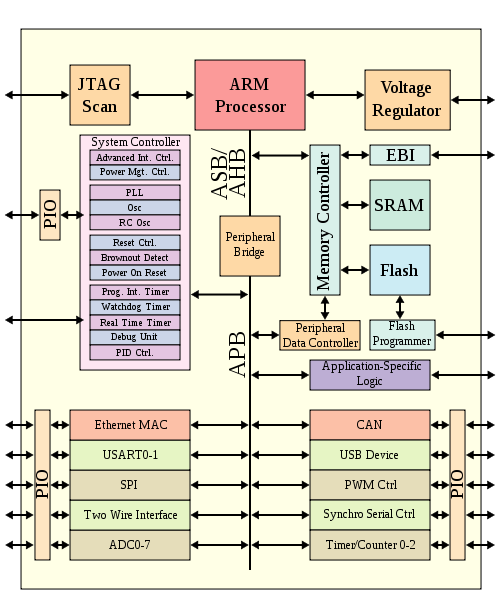
\includegraphics[scale=0.9]{ARMSoCBlockDiagram.png}
	\caption{Exemple de SoC}
\end{center}
\end{figure}

\clearpage

\subsection{ Les architectures x86 et x86-64 }

L'architecture x86(32 bits) ou x86-64(64 bits) sont les architectures les plus utilisées sur les ordinateurs aujourd'hui. Elles utilises les jeux d'instructions du type CISC (Complex instruction set computer). Ce type d'architecture comporte aussi des processeurs multi-cœurs mais aussi des processeurs utilisant l'hyper-threading que nous détaillerons dans les parties suivantes.

\subsubsection{ Complex instruction set computer }

Comme évoquer précédemment, cette architecture de processeur utilise des jeux d'instruction du type CISC utilisant de très nombreuses instructions mixées à des modes d'adressages complexes. \\
Ce type de jeu d'instructions possède plusieurs avantages :
\begin{itemize}
	\item L'empreinte mémoire du code est beaucoup plus dense. Par exemple on observe un facteur deux entre de l'ARM thumb et le x86). Cela pour effet de permettre l'utilisation minimale de la taille du cache instruction.
	\item Elle permet aussi de la microprogrammation, donc de corriger le jeu d'instructions. Cela facilite la correction de bug.
	\item Avec l'architecture CISC, on peut utiliser des instructions plus complexes non ou mal gérer par les compilateurs mais très rapide.
\end{itemize}
Ce type de microprocesseurs est plus difficile à accélérer. Leur structure est généralement plus complexe que sur une architecture RISC.

\subsubsection{ Hyper-threading }

Pour la réalisation de nos tests sur des machines d'architecture x86-64, 
nous rencontrerons l'hyper-threading. Développé par Intel, cela consiste schématiquement à doter un processeur de deux processeurs logiques sur une seule puce ayant, pour chacun, ses propres registres de données et de contrôle ainsi qu'un contrôleur d'interruption particulier. Ces deux unités partagent les éléments du cœur processeur, le bus système et le cache. Grâce à cette technologie, le processeur peut traiter deux sous processus simultanément. Au niveau des performances, cela ne remplace pas ceux d'un vrai cœur mais la présence de l'hyper-threading peut avoir une influence sur les futurs tests et donc sur les comparaisons. 

\section{ Les techniques de performances }

Dans cette section, nous allons lister plusieurs méthodes ou technologies de parallélisations ou de gain de performances pour les tests séquentiels que nous allons employer. Il existe certaines méthodes appartenant à un type d'architecture évoquer précédemment comme le SSE (Streaming SIMD Extensions) pour les processeurs x86-64 ou NEON (Advanced SIMD) les processeurs ARM.

\clearpage

\subsection{ L'utilisation des threads }

Un thread ou fil d'exécution est similaire à un processus dû à la même représentation de l'exécution d'un ensemble d'instructions du langage machine d'un processeur. Il permet, sur des machines à multi-cœurs, de paralléliser le traitement de calcul intensif car les threads ont la possibilité d'être exécutés chacun sur un cœur différent donc d'être réalisé au même moment. On retrouve l'utilisation des threads dans de nombreux langages de programmation comme le JAVA ou le C++ via la bibliothèque "pthread". Sur Android, elle est la principale méthode employée pour la parallélisation en programmation JAVA ou en natif. 

\subsection{ OpenMP (Open Multi-Processing) }

OpenMP est une interface de programmation conçue pour le calcul parallèle sur des architectures à mémoire partagée. Il se présente sous la forme d'un ensemble de directives, d'une bibliothèque logicielle et de variable d'environnement. Cette interface de programmation (API) présente plusieurs avantages. Il permet le développement d'applications parallèle rapidement tout en conservant un code proche du code séquentiel.
Un autre avantage est sa présence sur la plupart des systèmes d'exploitation comme Windows ou Unix. Depuis peu, il est possible de l'utiliser pour réaliser des programmes pour Android en natif.

\subsection{ MPI (Message Passing Interface) } 

MPI est une norme définissant une bibliothèque de fonctions conçue en 1993. Elle est utilisé dans les langages C, C++ et Fortran. Cette bibliothèque offre de bonnes performances aussi bien sur les machines à mémoires partagées que sur des machines à mémoire distribué (cluster). Par contre, elle nécessite plus de code qu'OpenMP de par la présence de paramètres pour le communicateur et pour l'exécution d'un type de communication (envoyer ou recevoir un message). Elle est disponible sur Windows et sur les systèmes UNIX mais elle n'est pas présente sur le système Android.

\subsection{ SSE (Streaming SIMD Extensions) }

SSE (Streaming (Single Instruction on Multiple Data) Extensions) est un jeu d'instructions supplémentaires pour microprocesseurs x86 et aujourd'hui les microprocesseurs x86-64. Elle introduit au processeur des instructions scalaires et de virgule flottante compactée. L'utilisation de ces instructions réduites le nombre d'instructions nécessaires à la réalisation d'un calcul utilisant des nombres flottants. Aujourd'hui cette technologie a reçu diverses mises à jour augmentant ces performances. Cette technologie n'est pas compatible avec l'architecture ARM mais celle-ci possède un équivalent assez proche nommé NEON (Advanced SIMD). 

\subsection{ NEON (Advanced SIMD) }





\subsection{ CUDA (Compute Unified Device Architecture) }

CUDA est une plate-forme de calcul parallèle et un modèle de programmation créé par NVIDIA. Cette technologie se différencie par l'utilisation des capacités de calcul d'un GPU (Graphics Processing Unit) afin d'accroitre les performances des ordinateurs et ainsi réaliser de calculs intensifs.    

 




 




\chapter{Analyse de l'existant}
\chapter{Besoins non fonctionnels}

\paragraph{}
	Notre domaine d'action se porte sur les appareils mobiles sous Android. Par extension notre hypothèse sera testée sur des ordinateurs.
\paragraph{}
	Nous n'avons aucune fiabilité sur la réussite de notre projet. Ce dernier étant un domaine de recherche, le but est d'affirmer ou de réfuter l'hypothèse énoncée précédemment.

\subsection*{Les algorithmes implémentés :\\}

\begin{itemize}

	\item Un bassin versant ou bassin-versant est une aire délimitée par des lignes de partage des eaux, à l'intérieur des quelles toutes les eaux tombées alimentent un même exutoire : cours d'eau, lac, mer, océan, etc. Une ligne de partage des eaux ce confond très souvent avec une ligne de crête.\\

	Chaque bassin versant se subdivise en un certain nombre de bassins élémentaires (parfois appelés « sous-bassin versant ») correspondant à la surface d'alimentation des affluents se jetant dans le cours d'eau principal.\\

	\item Il s'agit de la façon la plus fréquente de multiplier des matrices entre elles.\\
	En algèbre linéaire, une matrice A de dimensions m lignes et n colonnes (matrice m×n) représente une application linéaire f d'un espace de dimension n vers un espace de dimension m. Une matrice colonne V de n lignes est une matrice n×1, et représente un vecteur v d'un espace vectoriel de dimension n. Le produit A×V représente f(v).\\
	Si A et B représentent respectivement les applications linéaires f et g, alors A×B représente la composition des applications fog.\\
	Cette opération est utilisée notamment en mécanique lors des calculs de torseur statique, ou en informatique pour la matrice d'adjacence d'un graphe. \\
	Le produit de deux matrices ne peut se définir que si le nombre de colonnes de la première matrice est le même que le nombre de lignes de la deuxième matrice, c'est-à-dire lorsqu'elles sont de type compatible.

	\item  On peut trouver une valeur approchée de $\pi$ de façon empirique, en traçant un cercle, puis en mesurant son diamètre et sa circonférence, puis en divisant la circonférence par le diamètre. Une autre approche géométrique, attribuée à Archimède, consiste à calculer le périmètre Pn d’un polygone régulier à n côtés et à mesurer le diamètre d de son cercle circonscrit, ou celui de son cercle inscrit. Plus le nombre de côtés du polygone est grand, meilleure est la précision obtenue pour la valeur de $\pi$.\\
	Archimède a utilisé cette approche en comparant les résultats obtenus par la formule en utilisant deux polygones réguliers ayant le même nombre de côtés, pour lesquels le cercle est pour l’un circonscrit et pour l’autre inscrit. Il a réussi, avec un polygone à 96 côtés, à déterminer que 3 + 10/71 $< \pi <$ 3 + 1/7.\\
	On peut également obtenir des valeurs approchées de $\pi$ en mettant en œuvre des méthodes plus modernes. La plupart des formules utilisées pour calculer $\pi$ se basent sur la trigonométrie et le calcul intégral. Cependant, certaines sont particulièrement simples, comme la formule de Leibniz.

	\item l’histogramme représente la distribution des intensités d'une matrice.
	
\end{itemize}

	\subsection*{Langage d'implémentation :}
		Pour effectuer nos tests nous avons opté pour écrire un code natif, c'est-à-dire du C/C++ pour que le code soit portable autant sur appareils mobile que sur nos ordinateurs, en changeant un minimum l'implémentation. 

	\subsection*{Tests de validation :}
		Nous ne pouvons pas réellement prévoir de tests de validation, étant donné que nous ne savons pas encore quel genre de résultat nous allons obtenir; nous ne pourrons seulement valider nos tests que s'ils convergent vers le même résultat. 

	\subsection*{Description des problèmes associés :}
		Tout algorithme n'est pas parallélisable. En effet, induire du parallélisme peut ralentir le temps d'exécution d'un algorithme. En d'autres termes, un même algorithme peu être plus efficace en séquentielle qu'en parallèle.\\

		Produire du code parallèle pousse le développeur à avoir une vision différente des algorithmes. Le but du développeur ici est d'avoir le meilleur gain possible. Autrement dis le temps d'exécution d'un programme parallèle doit avoir un réel facteur de division du temps en fonction du nombre de coeurs choisie.

\chapter{Besoins fonctionnels}

\section{Le but}
\paragraph{}
	Le but de ce projet est d'établir l'utilité de la parallélisation dans un code, en vue de réduire la consommation énergétique d'une batterie d'un appareil mobile, par extension la consommation sur un ordinateur fixe ou portable. \\

	Les batteries d'appareils mobiles sont de plus en plus mal menées par les nouvelles applications qui consomment de plus en plus de batterie, sans que ces dernières n'évoluent. Il faut donc trouver d'autres solutions pour limiter la consommation excessive d'énergie.\\

	En parallèle les processeurs d'appareils mobiles eux évolue pour avoir de plus grandes cadences de calculs et être de plus en plus nombreux dans nos derniers appareilles multimédia.\\

	Par exemple, le Galaxy S4 de Samsung propose un Quad-core A15 (à 1.6GHz) plus un Quad-core A7 (à 1.2GHz), il serait donc dommage de ne pas exploiter cette puissance de calcule pour nos applications, tout en gardant un oeil sur la consomation énèrgetique. Les mêmes conceptes et même problématiques s'appliquent aux ordinateurs .\\

\section{L'application}
\paragraph{}
	L'idée est de déterminer si il vaut mieux effectuer un calcul sur un processeur avec une grande cadence de calcul ou de distribuer le calcul sur plusieurs processeurs plus lent, mais qui par conséquent consomme moins d'énergie. \\

	En effet un processeur, cadencé à 4GHz, consommerait plus que quatre processeurs, cadencés à 1Ghz, pourtant le temps de calcul devrait être sensiblement le même.\\

	Pour vérifier cette hypothèse nous allons réaliser différents tests avec différents calculs, sur plusieurs architectures; et ainsi déterminer si nous consommerions moins d'énergie en réduisant la fréquence du processeur dynamiquement et en répartissant les calculs sur les différents processeurs.\\

	En effet nous cherchons à déterminer si en distribuant un code la consommation énergétique diminue. Sachant que la consommation énergétique augmente de façon exponentielle.\\

	Pour moduler la fréquence et le voltage des appareils mobiles Android, nous nous sommes basé sur l'application AnTUTU\footnote{AnTUTU : \url{https://play.google.com/store/apps/details?id=com.antutu.CpuMasterFree&hl=fr}}, qui nous permet de régler de façon simple la fréquence des différents processeurs disponibles sur nos appareils.\\

	Des alternatives à AnTUTU existent, par exemple, Voltage Control\footnote{Voltage Control : \url{https://play.google.com/store/apps/details?id=com.darekxan.voltagecontrol}} qui réalise la même chose. \\

	Pour vérifier la consommation de batterie nous utilisons Battery Monitor\footnote{Battery Monitor : \url{https://play.google.com/store/apps/details?id=ccc71.bmw}}, cette application trace une courbe de la consommation batterie en direct, mais nous oblige à garde l'application ouverte en tache de fond ce qui utilisera aussi un peu de batterie et donc nos résultat seront légérement faussé mais la consommation engendrée par cette application devrait être négligeable dans nos résultats. \\

	Nous utiliserons aussi Battery Log\footnote{Battery Log : \url{https://play.google.com/store/apps/details?id=kr.hwangti.batterylog&hl=fr}} qui écrit dans un fichier les informations de la batterie à un instant T et l'intervalle entre deux temps est modulable.\\

	En ce qui concerne nos tests sur ordinateur nous travaillons sous linux avec l'outil CPUFreq-selector\footnote{CPUFreq-selector : \url{http://manpages.ubuntu.com/manpages/hardy/man1/cpufreq-selector.1.html}} qui nous permet, comme AnTUTU sous Android, de moduler la fréquence des processeurs.\\

	Ces outils nous permettrons d'évaluer les différents résultats obtenus durant nos tests.

\chapter{Résultats de tests}

\section{ L'experimentation de différents algorithmes parallèle sur ARM\footnote{Les architectures ARM, développées par ARM Ltd, sont dotés d'une architecture relativement plus simple que d'autres familles de processeurs, et bénéficiant d'une faible consommation, les processeurs ARM sont devenus dominants dans le domaine de l'informatique embarquée, en particulier la téléphonie mobile et les tablettes.} avec Android }

\paragraph{Les outils / Code parallèle \\}

	Il n'existe pas beaucoup d'outils pour paralléliser du code. Nous avons dû faire une recherche sur ce qui existe et utilisable sur Android (cf : 5-Besoins fonctionnels). \\

	Pour obtenir des gains de performance nous nous sommes penchés sur les librairies de parallèlisme classique. Parmi celles ci nos tests ont montrés qu'il était possible d'utiliser des technologies comme les Threads C++11, OpenMP et NEON\footnote{L'ARM NEON également appelé Advanced SIMD ou encore « MPE » (de l'anglais media processing engine, littéralement « moteur de calcul de médias ») est une unité de calcul de type SIMD(Single Instruction on Multiple Data), accélérant les calculs} pour la partie Android. En plus de ces technologies, les ordinateurs classiques nous permettent d'utiliser des technologies comme SSE\footnote{Streaming SIMD Extensions, généralement abrégé SSE, est un jeu de 70 instructions supplémentaires pour microprocesseurs x86, le fonctionnement est de type SIMD.}, AVX\footnote{Advanced Vector Extensions, est une extension  des instructions SSE et s'appliquent sur des registres deux fois plus grand.}, ou encore CUDA\footnote{CUDA (Compute Unified Device Architecture) est une technologie de GPGPU (General-Purpose Computing on Graphics Processing Units), c'est-à-dire qu'un processeur graphique (GPU) est utilisé pour exécuter des calculs généraux habituellement exécutés par le processeur central (CPU).}.\\

\paragraph{L'estimation des performances énergétiques \\}

	Le but est de tester la consommation énergetique du parallélisme sur Android et sur PC avec les différentes technologies exploitables. \\

	Nos tests consistent à exécuter des algorithmes où le parallélisme s'applique de façon optimale. Pour ce, des algorithmes où le parallélisme est maximal serait optimale, c'est-à-dire où chaque processeurs travailleraient sur des tailles de données équivalentes (cf : Non Fonctionnelle).

\begin{landscape}
\chapter{Planning}
\end{landscape}

\bibliographystyle{plain} % Le style est mis entre accolades.
\bibliography{bibli} % mon fichier de base de données s'appelle bibli.bib
\nocite{ref1, ref2, ref3, ref4, ref5, ref6, ref7, ref8, ref9, ref10, ref11, ref12, ref13, ref14, ref15, ref16, ref17, ref18, ref19, ref20, ref21, ref22, ref23, ref24}

\end{document} 